% Pengaturan ukuran teks dan bentuk halaman dua sisi
\documentclass[12pt]{book}

% Pengaturan ukuran halaman dan margin
\usepackage[a4paper,top=30mm,left=30mm,right=20mm,bottom=25mm]{geometry}

% Pengaturan ukuran spasi
\usepackage[singlespacing]{setspace}

% Pengaturan caption untuk tabel
\usepackage{caption}

% Judul dokumen
\title{Proposal Tugas Akhir ITS}
\author{Musk, Elon Reeve}

% Pengaturan detail pada file PDF
\usepackage[pdfauthor={\@author},bookmarksnumbered,pdfborder={0 0 0}]{hyperref}


% Pengaturan ukuran indentasi
\setlength{\parindent}{2em}

% Package lainnya
\usepackage{changepage}
\usepackage{etoolbox} % Mengubah fungsi default

% Pengaturan jenis karakter
\usepackage[utf8]{inputenc}

\usepackage[style=ieee, backend=biber]{biblatex}
\usepackage{enumitem} % Pembuatan list
\usepackage{lipsum} % Pembuatan template kalimat
\usepackage{graphicx} % Input gambar
\usepackage{longtable} % Pembuatan tabel
\usepackage[table,xcdraw]{xcolor} % Pewarnaan tabel
\usepackage{eso-pic} % Untuk menggunakan background image di halaman
\usepackage{txfonts} % Font times
\usepackage{changepage} % Pembuatan teks kolom
\usepackage{multicol} % Pembuatan kolom ganda
\usepackage{multirow} % Pembuatan baris ganda
\usepackage{tabularx} % Untuk mengatur kolom, seperti grid pada CSS
\usepackage{wrapfig}
\usepackage{float}

% Pengaturan format daftar isi, daftar gambar, dan daftar tabel
\usepackage[titles]{tocloft}
\setlength{\cftsecindent}{2em}
\setlength{\cftsubsecindent}{2em}
\setlength{\cftbeforechapskip}{1.5ex}
\setlength{\cftbeforesecskip}{1.5ex}
\setlength{\cftbeforetoctitleskip}{0cm}
\setlength{\cftbeforeloftitleskip}{0cm}
\setlength{\cftbeforelottitleskip}{0cm}
\renewcommand{\cfttoctitlefont}{\hfill\Large\bfseries} % command untuk membuat heading bold dan besar
\renewcommand{\cftaftertoctitle}{\hfill}
\renewcommand{\cftloftitlefont}{\hfill\Large\bfseries}
\renewcommand{\cftafterloftitle}{\hfill}
\renewcommand{\cftlottitlefont}{\hfill\Large\bfseries}
\renewcommand{\cftafterlottitle}{\hfill}

% Definisi untuk "Hati ini sengaja dikosongkan"
\patchcmd{\cleardoublepage}{\hbox{}}{
  \thispagestyle{empty}
  \vspace*{\fill}
  \begin{center}\textit{[Halaman ini sengaja dikosongkan]}\end{center}
  \vfill}{}{}

  % Pengaturan penomoran halaman
\usepackage{fancyhdr}
\fancyhf{}
\renewcommand{\headrulewidth}{0pt}
\pagestyle{fancy}
\fancyfoot[C,CO]{\thepage}
\patchcmd{\chapter}{plain}{fancy}{}{}
\patchcmd{\chapter}{empty}{plain}{}{}

% Pengaturan format judul bab
\usepackage{titlesec}
\renewcommand{\thesection}{\thechapter.\arabic{section}}
\titleformat{\chapter}[hang]{\centering\bfseries\large}{BAB\ \arabic{chapter}\ }{0ex}{\vspace{0ex}\centering}
\titleformat*{\section}{\large\bfseries}
\titleformat*{\subsection}{\normalsize\bfseries}
\titlespacing{\chapter}{0ex}{0ex}{4ex}
\titlespacing{\section}{0ex}{1ex}{0ex}
\titlespacing{\subsection}{0ex}{0.5ex}{0ex}
\titlespacing{\subsubsection}{0ex}{0.5ex}{0ex}
\setcounter{secnumdepth}{3} % Untuk memberi penomoran pada \subsubsection

\counterwithin{figure}{chapter}
\counterwithin{table}{chapter}

% Mengganti figure dan table menjadi gambar dan tabel
\renewcommand{\figurename}{Gambar}
\renewcommand{\tablename}{Tabel}

% Tambahkan format tanda hubung yang benar di sini
\hyphenation{
  ro-ket
  me-ngem-bang-kan
  per-hi-tu-ngan
}

% Menambahkan resource daftar pustaka
\addbibresource{pustaka/pustaka.bib}

% Isi keseluruhan dokumen
\begin{document}
  % Nomor halaman pembuka dimulai dari sini
  \pagenumbering{roman}

  % Atur ulang penomoran halaman
  \setcounter{page}{1}

  % Sampul Bahasa Indonesia
  \newcommand\covercontents{sampul/konten-id.tex}
  \AddToShipoutPictureBG*{
  \AtPageLowerLeft{
    % Ubah nilai berikut jika posisi horizontal background tidak sesuai
    \hspace{-3.25mm}

    % Ubah nilai berikut jika posisi vertikal background tidak sesuai
    \raisebox{0mm}{
      \includegraphics[width=\paperwidth,height=\paperheight]{sampul/gambar/sampul-luar-tipis.png}
    }
  }
}

% Menyembunyikan nomor halaman
\thispagestyle{empty}

% Pengaturan margin untuk menyesuaikan konten sampul
\newgeometry{
  top=65mm,
  left=30mm,
  right=30mm,
  bottom=20mm
}

\begin{flushleft}

  % Pemilihan font sans serif
  \sffamily

  % Pemilihan font bold
  \fontseries{bx}
  \selectfont
  \begin{spacing}{1.5}
    \input{\covercontents}
  \end{spacing}

\end{flushleft}

\restoregeometry


  % Lembar pengesahan
  \chapter*{LEMBAR PENGESAHAN}

% Menyembunyikan nomor halaman
\thispagestyle{empty}

\begin{center}
  % Ubah kalimat berikut dengan judul tugas akhir
  \textbf{KALKULASI ENERGI PADA ROKET LUAR ANGKASA BERBASIS \emph{ANTI-GRAVITASI}}
\end{center}

\begingroup
% Pemilihan font ukuran small
\small

\begin{center}
  % Ubah kalimat berikut dengan pernyataan untuk lembar pengesahan
  \textbf{PROPOSAL TUGAS AKHIR} \\
  Diajukan untuk memenuhi salah satu syarat memperoleh gelar
  Sarjana Teknik pada
  Program Studi S-1 Teknik Dirgantara \\
  Departemen Teknik Dirgantara \\
  Fakultas Teknik Dirgantara \\
  Institut Teknologi Sepuluh Nopember
\end{center}

\begin{center}
  % Ubah kalimat berikut dengan nama dan NRP mahasiswa
  Oleh: \textbf{Elon Reeve Musk} \\
  NRP. 0123 20 4000 0001
\end{center}

\begin{center}
  Disetujui Oleh:
\end{center}

\vspace{10ex}

\begingroup
% Menghilangkan padding
\setlength{\tabcolsep}{0pt}

\noindent
\begin{tabularx}{\textwidth}{X c}
  % Ubah kalimat-kalimat berikut dengan nama dan NIP dosen pembimbing pertama
  Nikola Tesla, S.T., M.T.      &                 \\
  NIP: 18560710 194301 1 001    & (Pembimbing)    \\
                                &                 \\
                                &                 \\
                                &                 \\
  % Ubah kalimat-kalimat berikut dengan nama dan NIP dosen pembimbing kedua
  Wernher von Braun, S.T., M.T. &                 \\
  NIP: 19230323 197706 1 001    & (Ko-Pembimbing) \\
\end{tabularx}
\endgroup

\vspace{\fill}

\begin{center}
  Mengetahui,\\
  % Ubah kalimat berikut dengan nama departemen
  Kepala Departemen Teknik Dirgantara FTD-ITS\\
  \vspace{10ex}
  % Ubah kalimat berikut dengan jabatan kepala departemen
  \underline{Nikola Tesla, S.T., M.T. }\\
  NIP 18560710 194301 1 001\\
  \vspace{10ex}
  % Ubah text dibawah menjadi tempat dan tanggal
  \textbf{SURABAYA} \\
  \textbf{Mei, 2077}
\end{center}
\endgroup

  \cleardoublepage

  % Abstrak
  \chapter*{ABSTRAK}
\begin{center}
  \large
  \textbf{KALKULASI ENERGI PADA ROKET LUAR ANGKASA BERBASIS \emph{ANTI-GRAVITASI}}
\end{center}
\addcontentsline{toc}{chapter}{ABSTRAK}
% Menyembunyikan nomor halaman
\thispagestyle{empty}

\begin{flushleft}
  \setlength{\tabcolsep}{0pt}
  \bfseries
  \begin{tabular}{ll@{\hspace{6pt}}l}
  Nama Mahasiswa / NRP&:& Elon Reeve Musk / 0123204000001\\
  Departemen&:& Teknik Dirgantara FTD - ITS\\
  Dosen Pembimbing&:& 1. Nikola Tesla, S.T., M.T.\\
  & & 2. Wernher von Braun, S.T., M.T.\\
  \end{tabular}
  \vspace{4ex}
\end{flushleft}
\textbf{Abstrak}

% Isi Abstrak
Abstrak harus berisi seratus hingga dua ratus kata. \lipsum[1]

\vspace{2ex}
\noindent
\textbf{Kata Kunci: \emph{Roket, Anti-gravitasi, Meong}}
  \cleardoublepage

  \chapter*{ABSTRACT}
\begin{center}
  \large
  \textbf{\emph{MINTING NFT ON SOLANA BLOCKCHAIN FOR MUSIC CONCERT TICKETS IN A MARKETPLACE USING SMART CONTRACTS BASED ON WEB3.0}}
\end{center}
% Menyembunyikan nomor halaman
\thispagestyle{empty}

\begin{flushleft}
  \setlength{\tabcolsep}{0pt}
  \bfseries
  \begin{tabular}{lc@{\hspace{6pt}}l}
  Student Name / NRP&: &Rianco Marcellino Andreas / 5024211061\\
  Department&: &Computer Engineering FTEIC - ITS\\
  Advisor&: &1. Mochamad Hariadi, S.T., M.Sc., Ph.D\\
  & & 2. Dr. Susi Juniastuti, S.T., M.Eng.\\
  \end{tabular}
  \vspace{4ex}
\end{flushleft}

\textbf{Abstract}

The music concert ticketing industry faces significant challenges related to ticket counterfeiting, illegal reselling, and lack of transparency. This research proposes the development of a minting system for Non-Fungible Tokens (NFTs) based on the \textit{Solana Blockchain} for music concert tickets, aiming to address these issues. The primary focus of this research is to optimize the NFT minting process to enhance the efficiency, security, and scalability of the digital ticketing system. The methodology includes designing and implementing \textit{smart contracts} on the \textit{Solana} platform, developing a \textit{Web3.0} interface for user interaction, and optimizing the minting process to reduce \textit{gas fees} and improve throughput. The proposed system is tested through high-load simulations and limited user trials to evaluate performance and usability. The expected outcomes include significant improvements in ticket security and authentication, more efficient secondary sales management, and an enhanced user experience in purchasing and utilizing digital concert tickets. This research also aims to provide insights into the integration of \textit{Solana Blockchain} and \textit{Web3.0} technologies within the entertainment industry. The key contribution of this research is the development of an optimized NFT minting system for music concert tickets, which has the potential to transform the management and distribution of digital tickets. The findings are expected to lay the foundation for broader adoption of \textit{blockchain} technology in ticketing and pave the way for further innovation in digital concert experiences.

\vspace{2ex}
\noindent
\textbf{Keywords: \emph{NFT, Solana Blockchain, Digital Concert Tickets, Smart Contracts, Web3.0, Minting Optimization}}

  \cleardoublepage

  \begin{spacing}{1.5}
    % Daftar isi
    \renewcommand*\contentsname{DAFTAR ISI}
    \addcontentsline{toc}{chapter}{\contentsname}
    \tableofcontents
    \cleardoublepage

    % Daftar gambar
    \renewcommand*\listfigurename{DAFTAR GAMBAR}
    \addcontentsline{toc}{chapter}{\listfigurename}
    \listoffigures
    \cleardoublepage

    % Daftar tabel
    \renewcommand*\listtablename{DAFTAR TABEL}
    \addcontentsline{toc}{chapter}{\listtablename}
    \listoftables
    \cleardoublepage
  \end{spacing}

  % Nomor halaman isi dimulai dari sini
  \pagenumbering{arabic}

  % Konten pendahuluan
  \chapter{PENDAHULUAN}

\section{Latar Belakang}

% Ubah paragraf-paragraf berikut sesuai dengan latar belakang dari tugas akhir
    

Perkembangan teknologi \textit{blockchain} telah membuka peluang baru dalam berbagai sektor, dengan \textit{Non-Fungible Tokens (NFT}) muncul sebagai inovasi yang menjanjikan, terutama dalam industri \textit{ticketing}, karya seni, dan koleksi digital. Pada proses pengerjaan \textit{minting} NFT merupakan penciptaan token unik didalam \textit{blockchain} agar menjadi aspek krusial dalam implementasi teknologi untuk tiket konser musik. Proses pengubahan tiket menjadi NFT dicatat secara permanen di \textit{blockchain}, memberikan bukti kepemilikan yang transparan dan tidak dapat dimanipulasi.

Wang \textit{et al.}  menegaskan bahwa proses \textit{minting NFT }menciptakan representasi digital unik dari aset, yang sangat relevan untuk tiket acara yang memiliki karakteristik \textit{non-fungible}\cite{ref1}. Fokus pada\textit{ minting} NFT adalah proses yang dapat menciptakan hubungan antara objek digital dan aset yang berada pada \textit{blockchain} dan dapat juga mengatasi masalah pemalsuan dimana diproyeksikan mencapai nilai \$31 miliar pada tahun 2022\cite{ref2}. Sebuah studi oleh Regner \textit{et al.}  dalam mendemonstrasikan bahwa \textit{minting} NFT untuk tiket dapat secara efektif mengatasi masalah pemalsuan dan penjualan kembali tiket ilegal, serta memungkinkan manajemen yang lebih baik atas penjualan sekunder\cite{ref3}

Implementasi sistem \textit{minting} NFT untuk tiket konser memerlukan pengembangan \textit{smart contract} yang \textit{sophisticated}. Caldarelli  dalam "Ledger" menekankan pentingnya desain \textit{smart contract} yang \textit{robust} untuk aplikasi \textit{blockchain}, termasuk dalam proses minting NFT\cite{ref4}.Dengan menggabungkan proses \textit{minting} NFT dengan teknologi \textit{Web3.0}, ada peluang untuk meningkatkan efisiensi dan kemudahan akses sistem. Menurut Zou \textit{et al.} dalam "IEEE Internet of Things Journal", \textit{Web3.0 }dapat meningkatkan keamanan dan interoperabilitas sistem \textit{berbasis} \textit{blockchain}\cite{ref5}

Meskipun demikian, implementasi sistem \textit{minting} NFT untuk tiket konser menghadapi beberapa tantangan teknis. Chittoda dan Ghosh dalam konferensi ICACCCN mengidentifikasi masalah skalabilitas dan biaya transaksi sebagai hambatan utama dalam proses minting dan adopsi luas NFT \cite{ref6}. Optimasi proses minting menjadi krusial untuk mengatasi tantangan ini. Selain itu aspek hukum menjadi pertimbangan yang baik, Kugler dalam "Komunikasi ACM" membahas masalah teknis dan hukum yang terkait dengan minting dan penggunaan NFT, menekankan betapa pentingnya membangun protokol \textit{minting} yang efektif dan sesuai dengan peraturan\cite{ref7}. Hal ini menjadi tantangan dalam pengembangan sistem \textit{ticketing} NFT yang dapat diadopsi secara luas. 

Oleh karena itu, tujuan dari penelitian ini adalah untuk mengembangkan dan menerapkan sistem \textit{minting} NFT yang aman dan efisien untuk tiket konser musik dalam lingkungan \textit{marketplace} berbasis \textit{Web3.0}. Fokus utama akan diberikan pada optimasi proses \textit{minting}, termasuk kecepatan, biaya, dan keamanan. Pengembangan \textit{smart contract} yang kuat untuk \textit{minting} dan integrasi lancar dengan teknologi \textit{Web3.0} akan menjadi komponen utama penelitian ini. Hasil penelitian ini diharapkan dapat memberikan kontribusi yang signifikan terhadap perkembangan sistem \textit{ticketing} digital dan mendorong adopsi teknologi \textit{blockchain} dalam industri hiburan yang lebih luas. Dengan mengatasi tantangan teknis dan menawarkan solusi yang efektif, penelitian ini berpotensi mentransformasi cara tiket konser musik dikelola, didistribusikan, dan digunakan, membuka jalan bagi inovasi lebih lanjut dalam pengalaman konser digital.

\section{Rumusan Masalah}

Berdasarkan hal yang telah dipaparkan di latar belakang, didapatkan bahwa permasalahan yang ada pada masalah riset ini yaitu :
\begin{enumerate}
    \item Bagaimana merancang sistem minting NFT untuk tiket konser musik menggunakan Solana Blockchain yang dapat memastikan setiap tiket memiliki atribut unik, seperti identitas pemilik, nomor kursi, dan tanggal konser?
    \item Bagaimana mengimplementasikan integrasi antara smart contract pada Solana Blockchain dan web berbasis Web3.0 untuk  minting , pembelian, dan transfer tiket konser dalam bentuk NFT?
    \item Bagaimana membangun marketplace berbasis NFT yang memungkinkan pengguna untuk membuat, membeli, dan menjual aset digital menggunakan teknologi blockchain?
\end{enumerate}



\section{Batasan Permasalahan}

Dalam pengembangan sistem marketplace berbasis \textit{blockchain} untuk minting NFT tiket konser musik, batasan permasalahan yang ditetapkan adalah sebagai berikut:

\begin{enumerate}
    \item \textbf{Teknologi Blockchain:}
    \begin{itemize}
        \item Sistem ini menggunakan \textit{Solana Blockchain} sebagai infrastruktur utama untuk transaksi dan pencatatan NFT.
        \item Transaksi hanya dilakukan pada jaringan \textit{Devnet} untuk tujuan pengembangan dan pengujian, bukan pada jaringan \textit{Mainnet}.
    \end{itemize}

    \item \textbf{NFT (Non-Fungible Token):}
    \begin{itemize}
        \item NFT yang dihasilkan merepresentasikan tiket konser musik dengan metadata seperti nama acara, lokasi, tanggal, waktu, dan kategori tiket (VIP, reguler).
        \item \textit{Minting NFT} dilakukan melalui integrasi \textit{smart contract} yang telah diimplementasikan sesuai dengan protokol Solana.
    \end{itemize}

    \item \textbf{Marketplace:}
    \begin{itemize}
        \item Marketplace ini hanya mendukung fungsi dasar seperti minting, penjualan, dan pembelian tiket berbasis NFT.
        \item Transaksi dilakukan menggunakan mata uang kripto \textit{SOL}.
    \end{itemize}

    \item \textbf{Dompet Digital:}
    \begin{itemize}
        \item Sistem hanya mendukung dompet digital \textit{Phantom Wallet} untuk autentikasi pengguna, transaksi, dan penyimpanan NFT.
    \end{itemize}
    \item \textbf{Platform dan Teknologi:}
    \begin{itemize}
        \item {Frontend:} Dibangun menggunakan \textit{Next.js} dengan integrasi \textit{Web3.js} untuk komunikasi dengan blockchain.
        \item {Backend:} Backend dengan fungsionalitas terbatas yang mendukung proses \textit{minting NFT} dan penyimpanan metadata.
        \item Sistem tidak memiliki fitur analitik, manajemen pengguna, atau integrasi pihak ketiga di luar blockchain Solana.
    \end{itemize}

\end{enumerate}



\section{Tujuan}

Penelitian ini bertujuan untuk merancang dan mengimplementasikan sistem \textit{minting NFT tickets} berbasis \textit{Solana Blockchain} untuk memastikan keaslian tiket konser musik dengan memanfaatkan teknologi \textit{Web3.0}.

\section{Manfaat}

Penelitian ini memberikan manfaat sebagai berikut:
\begin{enumerate}
    \item Mencegah pemalsuan tiket konser melalui sistem verifikasi berbasis \textit{blockchain}.
    \item Meningkatkan transparansi dalam pencatatan riwayat kepemilikan tiket.
    \item Sistem ini memberikan panduan teknis bagi pengembang dalam membangun marketplace NFT yang mencakup proses minting, penyimpanan metadata, dan koneksi dengan dompet digital seperti Phantom Wallet.
    \item Penelitian ini juga berkontribusi pada pengembangan ekosistem blockchain dengan memanfaatkan jaringan Solana, yang dikenal dengan biaya transaksi rendah dan kecepatan tinggi, sehingga mendukung penerapan NFT dalam industri hiburan.
\end{enumerate}
  \cleardoublepage

  % Konten tinjauan pustaka
  \setlength{\parindent}{1cm}    % Untuk indentasi paragraf
\setlength{\parskip}{1em}      % Untuk jarak antar paragraf
% Di awal dokumen, tambahkan
\sloppy  % Membuat LaTeX lebih toleran terhadap spacing
\chapter{TINJAUAN PUSTAKA}

\section{Penelitian Terdahulu}

\subsection{Non-Fungible Token (NFT)}
Wang \textit{et al.} melakukan penelitian komprehensif tentang NFT yang menyoroti peluang dan tantangan dalam implementasinya. Penelitian ini memberikan pemahaman mendalam tentang teknologi NFT dan potensinya dalam berbagai aplikasi digital. Studi ini juga menganalisis aspek teknis NFT yang dapat dimanfaatkan untuk sistem tiket digital, termasuk mekanisme verifikasi dan keamanan \parencite{ref1}.

\subsection{NFT Implementation in Event Ticketing Systems}
Regner \textit{et al.} melakukan penelitian tentang implementasi NFT dalam sistem ticketing berbasis blockchain. Penelitian ini menganalisis bagaimana NFT dapat menjadi komponen kunci dalam sistem tiket event, dengan fokus pada aspek verifikasi dan pencegahan pemalsuan. Studi ini juga membahas bagaimana \textit{smart contract} dapat digunakan untuk mengotomatisasi proses ticketing dan memastikan keabsahan tiket \parencite{ref3}.

\subsection{Web3.0 Integration with Blockchain Systems}
Zou \textit{et al.} meneliti tentang visi masa depan internet dengan Web3.0 dan integrasinya dengan teknologi blockchain. Penelitian ini memberikan wawasan tentang bagaimana Web3.0 dapat meningkatkan interoperabilitas dan \textit{user experience} dalam aplikasi blockchain, termasuk sistem NFT ticketing \parencite{ref5}.

\subsection{Interoperabilitas NFT pada Web3.0}
Azis melakukan penelitian tentang interoperabilitas NFT berbasis blockchain menggunakan \textit{smart contract} pada Web3.0. Penelitian ini membahas bagaimana \textit{smart contract} dapat diimplementasikan untuk memungkinkan interoperabilitas antar NFT dalam lingkungan Web3.0. Studi ini memberikan kontribusi penting dalam pemahaman tentang pengembangan sistem NFT yang dapat berinteraksi lintas platform \parencite{ref8}.

\section{Dasar Teori}
% ====================
% Bagian Blockchain
% ====================
\subsection{Blockchain}
Blockchain merupakan teknologi basis data terdistribusi yang mengizinkan data disimpan dalam serangkaian blok yang terkoneksi. Setiap blok mengandung rangkaian transaksi yang sudah divalidasi, dan setiap pemantauan blok baru ke dalam rantai menjamin keabadian dan ketidakmampuan modifikasi dari transaksi yang tercatat. Fitur keamanan dan keterbukaan menjadi ciri khas blockchain, di mana setiap transaksi divalidasi oleh jaringan partisipan dan tercatat dalam rantai yang tak bisa dimodifikasi \parencite{ref1}.

Blockchain memiliki karakteristik utama sebagai berikut:
\begin{enumerate}
    \item \textit{Desentralisasi}: Mengeliminasi kebutuhan akan server pusat yang mengurangi biaya dan meningkatkan efisiensi.
    \item \textit{Ketahanan}: Menjamin bahwa setelah data dimasukkan dan dikonfirmasi, data tersebut hampir mustahil dihapus atau dimodifikasi.
    \item \textit{Anonimitas}: Menjaga identitas pengguna tetap anonim.
    \item \textit{Auditabilitas}: Semua transaksi dapat diaudit oleh pihak yang berwenang.
\end{enumerate}

\begin{figure}[H]
    \centering
    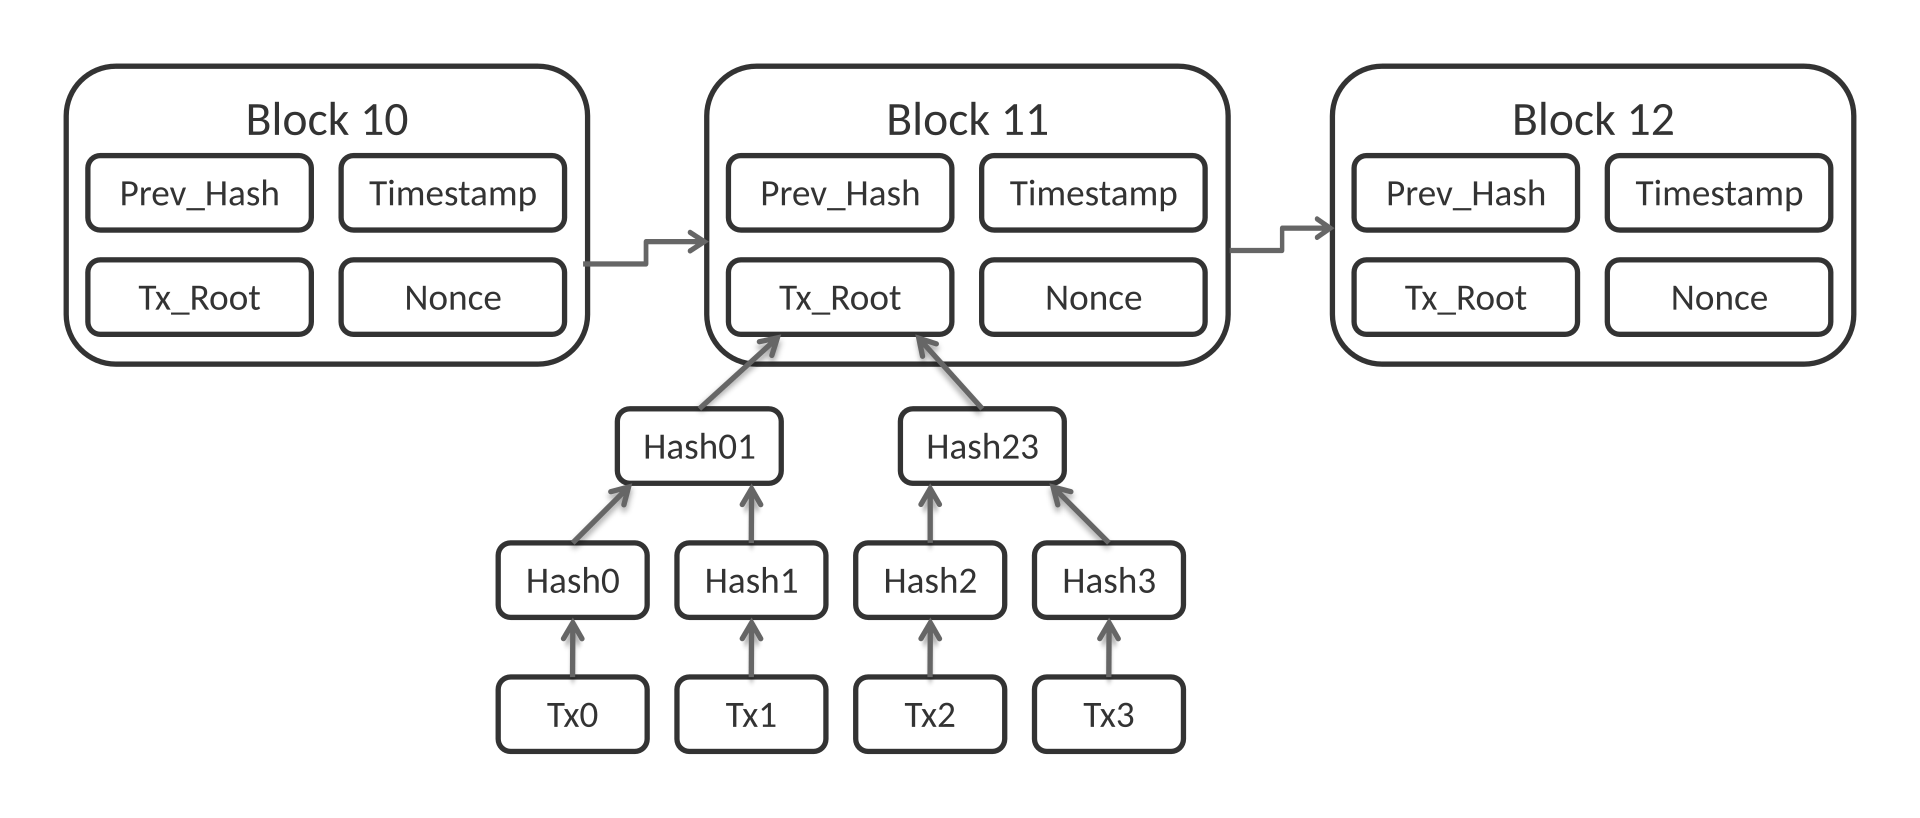
\includegraphics[width=0.8\textwidth]{gambar/2.2.1.png}
    \caption{Struktur Dasar Blockchain \parencite{ref1}}
    \label{fig:blockchain-structure}
\end{figure}

Blockchain terdiri dari beberapa komponen utama:
\begin{enumerate}
    \item Header: Berisi informasi seperti \textit{Block Version}, \textit{Merkle Tree Root Hash}, \textit{Timestamp}, dan \textit{Parent Block Hash}.
    \item Transaction Counter: Menunjukkan jumlah transaksi dalam blok.
    \item Transaksi: Berisi transaksi lengkap yang tercatat.
\end{enumerate}

Dalam perkembangannya, blockchain telah berkembang melampaui cryptocurrency dan kini digunakan dalam berbagai aplikasi, termasuk \textit{smart contract}, NFT, dan sistem ticketing terdesentralisasi. Keunggulan blockchain dalam hal transparansi, immutability, dan keamanan membuatnya ideal untuk aplikasi yang membutuhkan kepercayaan dan verifikasi tanpa pihak ketiga \parencite{ref3}.

% ====================
% Bagian Solana Blockchain  
% ====================
\subsection{Solana Blockchain}
Solana adalah platform blockchain \textit{high-performance} yang dirancang untuk mendukung aplikasi terdesentralisasi dan NFT. Platform ini menggunakan mekanisme konsensus \textit{Proof of History (PoH)} yang terintegrasi dengan \textit{Tower BFT}, memungkinkan throughput transaksi tinggi hingga 65.000 TPS dengan biaya transaksi yang sangat rendah \parencite{ref9}.

Keunggulan arsitektur Solana meliputi:
\begin{enumerate}
    \item Kecepatan Transaksi: Memungkinkan proses transaksi yang sangat cepat dengan throughput tinggi.
    \item Biaya Rendah: Biaya transaksi jauh lebih murah dibandingkan blockchain lainnya.
    \item Skalabilitas: Dapat menangani volume transaksi besar tanpa memperlambat jaringan.
    \item Keamanan: Memanfaatkan \textit{Tower BFT} untuk memastikan konsensus yang aman.
\end{enumerate}

\begin{figure}[H]
    \centering
    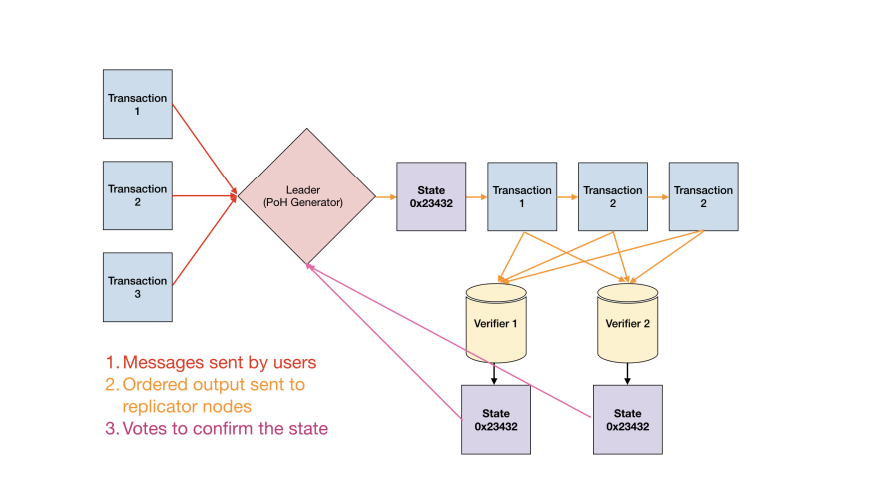
\includegraphics[width=0.8\textwidth]{gambar/2.2.2.png}
    \caption{Arsitektur Tower BFT Solana \parencite{ref9}}
    \label{fig:solana-tower-bft}
\end{figure}

Dalam arsitektur ini, node validator memiliki tanggung jawab berikut:
\begin{enumerate}
    \item Memproses transaksi yang masuk.
    \item Memberikan \textit{vote} untuk setiap \textit{state} yang valid.
    \item Berpartisipasi dalam konsensus jaringan.
    \item Menjaga sinkronisasi dengan \textit{state} terbaru.
\end{enumerate}

% ====================
% Bagian Smart Contract
% ====================
\subsection{Smart Contract}
\textit{Smart Contract} adalah protokol transaksi yang diotomatisasi, yang melaksanakan syarat-syarat dalam suatu perjanjian. Ketika suatu kondisi tertentu dipenuhi, \textit{smart contract} akan otomatis tereksekusi. \textit{Smart contract} dibuat di atas blockchain, di mana setiap eksekusi pernyataan kontrak dicatat sebagai transaksi yang tidak dapat diubah \parencite{ref1}.

Dalam ekosistem Solana, \textit{smart contract} dikenal sebagai \textit{Programs}. Program pada Solana dikembangkan menggunakan bahasa pemrograman \textit{Rust}, yang dipilih karena keunggulannya dalam hal keamanan memori dan performa tinggi. Setiap program di Solana memiliki alamat unik dan dapat dipanggil melalui transaksi atau oleh program lain \parencite{ref9}.

Keunggulan model \textit{stateless} pada Solana meliputi:
\begin{enumerate}
    \item Eksekusi paralel dari transaksi.
    \item Penggunaan memori yang lebih efisien.
    \item Biaya transaksi yang lebih rendah.
\end{enumerate}

% ====================
% Bagian SPL Token Standard
% ====================
% ====================
% Bagian SPL Token Standard
% ====================
\subsection{SPL Token Standard}

SPL (\textit{Solana Program Library}) Token Standard adalah standar token yang digunakan dalam ekosistem Solana untuk menciptakan dan mengelola token digital. SPL Token setara dengan ERC-20 pada Ethereum, tetapi memanfaatkan keunggulan arsitektur Solana seperti biaya transaksi rendah, throughput tinggi, dan efisiensi eksekusi. Fungsi utama yang didukung SPL Token meliputi transfer token, pencetakan atau \textit{minting} token baru, pembakaran atau \textit{burning} token, serta verifikasi saldo dalam akun. Model berbasis akun yang diterapkan oleh SPL Token memastikan bahwa saldo token hanya dapat diakses oleh pemilik akun atau program yang diberi izin.

Dalam proses penciptaan SPL Token, langkah pertama adalah membuat \textit{Mint Account} yang berfungsi untuk mencatat informasi dasar token seperti nama, simbol, dan jumlah maksimal token yang dapat dicetak. Setelah itu, metadata tambahan seperti nama token, deskripsi, dan properti lainnya dapat ditambahkan menggunakan standar Metaplex. Setelah metadata ditambahkan, pengguna perlu menciptakan \textit{Token Account} yang digunakan untuk menyimpan saldo token mereka. Terakhir, proses \textit{minting} dilakukan dengan mencetak token baru ke dalam \textit{Token Account} yang telah dibuat.

SPL Token memiliki beberapa keunggulan dibandingkan standar token lain. Biaya transaksi yang sangat rendah membuat SPL Token lebih ekonomis untuk digunakan dalam berbagai aplikasi, terutama untuk transaksi volume tinggi. Selain itu, kecepatan transaksi yang tinggi memungkinkan SPL Token untuk diproses secara efisien bahkan dalam kondisi jaringan yang sibuk. Standar ini juga menawarkan interoperabilitas yang baik, di mana SPL Token dapat digunakan oleh berbagai program atau \textit{smart contract} lain dalam ekosistem Solana.

Dalam konteks penelitian ini, SPL Token digunakan sebagai basis untuk menciptakan sistem tiket konser berbasis blockchain yang aman dan efisien. Keunggulan SPL Token dalam hal kecepatan, biaya rendah, dan interoperabilitas menjadi fondasi penting untuk mendukung implementasi sistem tiket digital yang memanfaatkan teknologi blockchain. Dengan menggunakan SPL Token, penelitian ini diharapkan dapat memberikan solusi inovatif dalam pengelolaan tiket konser digital.


% ====================
% Bagian Non-Fungible Token (NFT)
% ====================
\subsection{Non-Fungible Token (NFT)}

Non-Fungible Token (NFT) adalah token digital unik yang merepresentasikan kepemilikan aset digital atau fisik yang diverifikasi melalui blockchain. NFT berbeda dari token \textit{fungible} seperti cryptocurrency karena setiap NFT memiliki karakteristik unik yang tidak dapat digantikan atau dipertukarkan.

Proses pembuatan NFT pada Solana, yang dikenal sebagai \textit{minting}, melibatkan langkah-langkah berikut:
\begin{enumerate}
    \item {Membuat Mint Account}: Digunakan untuk mencatat properti unik NFT, seperti ID unik dan metadata dasar.
    \item {Menambahkan Metadata}: Informasi tambahan seperti nama, deskripsi, gambar, atau atribut khusus lainnya ditambahkan melalui standar Metaplex.
    \item {Menciptakan Token Account}: Akun yang dimiliki pengguna untuk menyimpan NFT mereka.
\end{enumerate}

Keunggulan NFT pada Solana meliputi:
\begin{enumerate}
    \item Biaya Rendah: Minting dan transfer NFT di Solana memiliki biaya yang jauh lebih rendah dibandingkan platform lain seperti Ethereum.
    \item Kecepatan Transaksi Tinggi: NFT dapat dibuat dan ditransfer dalam hitungan detik.
    \item Standarisasi Metadata: Standar Metaplex memungkinkan interoperabilitas dan konsistensi metadata NFT.
    \item Dukungan untuk Koleksi Besar: Solana mendukung pembuatan dan manajemen koleksi NFT dalam skala besar.
\end{enumerate}

NFT pada Solana menggunakan standar Metaplex untuk mendefinisikan metadata. Standar ini menyediakan format terstruktur untuk menyimpan informasi seperti:
\begin{enumerate}
    \item Nama dan deskripsi aset.
    \item URL ke file digital (gambar, video, atau dokumen).
    \item Properti tambahan seperti warna, ukuran, atau atribut lainnya.
\end{enumerate}



Dalam konteks penelitian ini, NFT digunakan sebagai representasi tiket konser digital. Dengan menggunakan SPL Token Standard dan standar Metaplex, sistem NFT memungkinkan:
\begin{enumerate}
    \item Verifikasi kepemilikan tiket secara real-time.
    \item Pencatatan riwayat transfer tiket untuk transparansi penuh.
    \item Pencegahan pemalsuan tiket melalui keunikan setiap NFT.
\end{enumerate}

Integrasi NFT dengan \textit{smart contract} dan Web3.0 pada Solana membuka peluang untuk mengembangkan sistem tiket digital yang aman, cepat, dan efisien.


% ====================
% Bagian Token Metadata
% ====================
\subsection{Token Metadata}

Token Metadata pada ekosistem Solana adalah standar yang digunakan untuk menyimpan dan mengelola informasi tambahan pada SPL Tokens, termasuk Non-Fungible Tokens (NFT). Metadata memungkinkan token untuk memiliki informasi deskriptif seperti nama, deskripsi, gambar, dan properti tambahan lainnya. Standar ini dikelola oleh Metaplex Foundation dan menjadi fondasi utama untuk penerapan NFT yang interoperabel di ekosistem Solana.\\

Proses pembuatan metadata melibatkan langkah-langkah berikut: 
Token metadata dibuat sebagai akun khusus di blockchain Solana yang menyimpan informasi deskriptif tentang token. Metadata ini dirancang untuk menyimpan data seperti:
\begin{enumerate}
    \item Nama dan deskripsi
    \item Simbol: Simbol singkat untuk token
    \item Tautan ke file JSON yang menyimpan metadata tambahan
\end{enumerate}


Token Metadata juga memungkinkan pengembang untuk menambahkan properti tambahan seperti:
\begin{enumerate}
    \item Atribut unik (misalnya warna, ukuran, atau properti lain)
    \item Tautan ke file digital (gambar, video, atau dokumen)
\end{enumerate}

Metadata token di Solana mengikuti format standar JSON yang terhubung dengan metadata akun di blockchain. Format JSON memungkinkan integrasi lintas platform, memastikan NFT dapat digunakan dalam aplikasi Web3.0 lainnya. Berikut adalah contoh struktur JSON metadata:
\begin{verbatim}
{
    "name": "NFT Contoh",
    "symbol": "NFTC",
    "description": "NFT unik dengan atribut warna biru.",
    "image": "https://link-ke-gambar.com/nftc.png",
    "attributes": [
        {
            "trait_type": "Warna",
            "value": "Biru"
        },
        {
            "trait_type": "Ukuran",
            "value": "Besar"
        }
    ]
}
\end{verbatim}

Token Metadata pada Solana memiliki beberapa keunggulan, termasuk biaya rendah, interoperabilitas, dan kecepatan tinggi. Standar ini digunakan secara luas dalam aplikasi NFT seperti marketplace digital, game berbasis blockchain, dan koleksi seni digital. Dengan mengikuti standar yang ditentukan oleh Metaplex Foundation, metadata token dapat dengan mudah diakses dan digunakan oleh aplikasi lain dalam ekosistem Solana.

\begin{figure}[H]
    \centering
    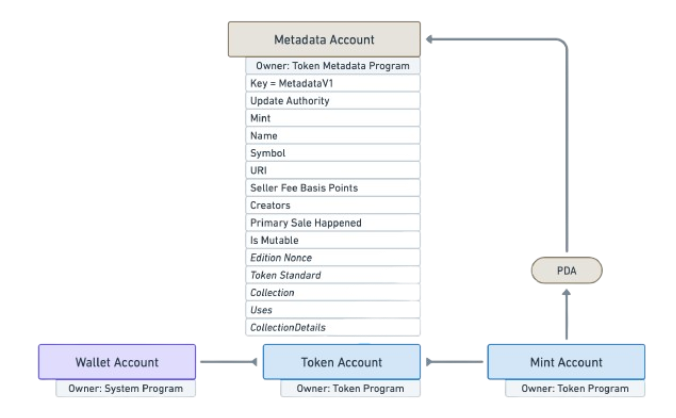
\includegraphics[width=0.8\textwidth]{gambar/2.2.4.png}
    \caption{Struktur Token Metadata pada Solana \parencite{ref10}}
    \label{fig:token-metadata}
\end{figure}

Dalam konteks penelitian ini, Token Metadata digunakan untuk menyimpan informasi tambahan tentang tiket konser digital. Metadata ini mencakup informasi seperti nama konser, nama artis, tanggal acara, dan lokasi. Standar ini memungkinkan sistem tiket berbasis blockchain untuk memberikan pengalaman pengguna yang lebih kaya dan terintegrasi.

% ====================
% Bagian Metaplex
% ====================
\subsection{Metaplex}
Metaplex adalah framework standar pada blockchain Solana yang menyediakan tools dan protokol untuk membuat, menerbitkan, dan mengelola NFT. Framework ini dikembangkan oleh Metaplex Foundation untuk memberikan standarisasi dalam pembuatan dan pengelolaan NFT pada ekosistem Solana \parencite{ref10}.

Metaplex terdiri dari beberapa komponen utama:
\begin{enumerate}[noitemsep,topsep=0pt]  % Ini akan mengurangi spasi
    \item Token Metadata Program: Mengelola metadata NFT
    \item Candy Machine: Program untuk minting NFT secara massal
    \item Auction House: Program untuk marketplace NFT
    \item Token Vault: Penyimpanan token yang aman
\end{enumerate}

Format metadata yang digunakan oleh Metaplex mengikuti standar JSON tertentu:

\begin{verbatim}
{
   "name": "NFT Contoh",
   "symbol": "NFTC",
   "description": "NFT unik dengan atribut warna biru.",
   "image": "https://link-ke-gambar.com/nftc.png",
   "attributes": [
       {
           "trait_type": "Warna",
           "value": "Biru"
       },
       {
           "trait_type": "Ukuran",
           "value": "Besar"
       }
   ]
}
\end{verbatim}


Dalam konteks pengembangan sistem tiket NFT, Metaplex menyediakan beberapa keunggulan:
\begin{enumerate}
   \item Standarisasi format metadata tiket
   \item Sistem minting yang efisien dan terukur
   \item Integrasi dengan wallet dan marketplace
   \item Kemampuan verifikasi dan validasi tiket
\end{enumerate}


% ====================
% Bagian IPFS (InterPlanetary File System)
% ====================
\subsection{IPFS (InterPlanetary File System)}
\textit{InterPlanetary File System} (IPFS) adalah sistem file \textit{peer-to-peer} terdistribusi yang dirancang untuk menyimpan dan mengakses file, \textit{website}, aplikasi, dan data dengan cara yang lebih efisien dan terdesentralisasi. IPFS menyediakan infrastruktur untuk menyimpan metadata secara permanen dan dapat diakses secara global \parencite{ref12}.

IPFS menggunakan model pengalamatan konten berbasis \textit{hash} kriptografis, di mana setiap file yang disimpan di IPFS akan mendapatkan \textit{Content Identifier} (CID) yang unik. CID ini berfungsi sebagai alamat permanen untuk mengakses konten dan tidak dapat diubah tanpa mengubah alamatnya. Keunikan sistem ini terletak pada kemampuannya untuk memverifikasi integritas data secara otomatis melalui \textit{hash} yang dihasilkan, sehingga setiap perubahan pada konten akan terdeteksi.

Dalam implementasinya, IPFS menggunakan teknologi \textit{Distributed Hash Table} (DHT) untuk mengatur penyimpanan dan pencarian konten dalam jaringan \textit{peer-to-peer}. Sistem ini memungkinkan file yang sama untuk tersedia di berbagai \textit{node} dalam jaringan, meningkatkan redundansi dan kecepatan akses. Ketika sebuah file diminta, IPFS akan mencari \textit{node} terdekat yang memiliki salinan file tersebut, mengoptimalkan waktu pengambilan dan mengurangi beban jaringan.

Dalam konteks NFT \textit{ticketing}, IPFS memainkan peran krusial dalam penyimpanan metadata tiket. Metadata ini mencakup detail acara seperti nama artis, tanggal pertunjukan, lokasi \textit{venue}, dan informasi penting lainnya. Penggunaan IPFS memastikan bahwa informasi tiket tetap tersedia dan tidak dapat dimanipulasi, memberikan tingkat keamanan tambahan dalam sistem \textit{ticketing} digital.

Proses integrasi IPFS dengan sistem NFT \textit{ticketing} melibatkan beberapa tahap penting. Pertama, metadata tiket dibuat dalam format JSON yang terstandarisasi. Kemudian, file ini diunggah ke jaringan IPFS, menghasilkan CID unik yang akan disimpan dalam \textit{smart contract} NFT. Ketika tiket perlu diverifikasi, sistem dapat mengakses metadata melalui CID ini, memastikan keaslian dan validitas tiket.

Keunggulan penggunaan IPFS dalam sistem NFT \textit{ticketing} tidak hanya terletak pada aspek keamanan, tetapi juga pada efisiensi dan skalabilitasnya. Sistem ini mampu menangani volume data yang besar dengan tetap mempertahankan kecepatan akses, sambil memberikan jaminan ketersediaan data yang tinggi melalui jaringan terdistribusinya.

% ====================
% Bagian Rust Programming Language
% ====================
\subsection{Rust Programming Language}
\textit{Rust Programming Language} adalah bahasa pemrograman sistem yang dikembangkan oleh Mozilla Research. Rust dirancang untuk menjadi bahasa pemrograman yang aman, konkuren, dan praktis. Dalam ekosistem Solana, Rust dipilih sebagai bahasa utama untuk pengembangan \textit{smart contract} karena keunggulannya dalam hal keamanan memori dan performa tinggi \parencite{ref13}.

Rust memiliki beberapa karakteristik utama yang membuatnya ideal untuk pengembangan program Solana. Sistem \textit{ownership} dan \textit{borrowing} pada Rust memastikan keamanan memori tanpa memerlukan \textit{garbage collector}, yang sangat penting dalam lingkungan blockchain di mana kesalahan memori dapat berakibat fatal. Selain itu, Rust mendukung pemrograman konkuren yang aman melalui fitur \textit{zero-cost abstractions} dan kontrol memori yang ketat.

Dalam konteks pengembangan program Solana, Rust menyediakan beberapa fitur penting:
\begin{enumerate}[noitemsep,topsep=0pt]
   \item Tipe data statis yang kuat untuk mencegah kesalahan runtime
   \item Penanganan error yang komprehensif melalui tipe Result
   \item \textit{Pattern matching} untuk pemrosesan data yang aman
   \item \textit{Cross-compilation} untuk berbagai target arsitektur
\end{enumerate}

Pengembangan program pada Solana menggunakan Rust mengikuti pola tertentu di mana setiap program harus mengimplementasikan trait \textit{Entrypoint} dan memiliki fungsi \textit{process\_instruction} sebagai titik masuk utama. Program ini kemudian dikompilasi menjadi \textit{Berkley Packet Filter} (BPF) \textit{bytecode} yang dapat dieksekusi oleh Solana \textit{runtime}.

Keamanan dalam pemrograman Rust untuk Solana sangat penting mengingat sifat permanen dari \textit{smart contract} yang sudah di-\textit{deploy}. Rust membantu mencegah berbagai jenis kerentanan umum melalui sistem tipe yang ketat dan pemeriksaan waktu kompilasi. Ini termasuk pencegahan \textit{buffer overflow}, \textit{race conditions}, dan kesalahan pengelolaan memori lainnya.

% ====================
% Bagian Web 3.0
% ====================
\subsection{Web 3.0}
\textit{Web} 3.0 merupakan generasi baru dari \textit{World Wide Web} yang menekankan pada desentralisasi dan \textit{blockchain} sebagai infrastruktur utamanya. Berbeda dengan \textit{Web} 2.0 yang berfokus pada interaksi sosial dan konten yang dihasilkan pengguna, \textit{Web} 3.0 memungkinkan interaksi langsung antar pengguna tanpa memerlukan perantara terpusat \parencite{ref5}.

Dalam konteks pengembangan aplikasi, \textit{Web} 3.0 menawarkan paradigma baru dimana aplikasi dibangun di atas jaringan terdesentralisasi. Hal ini memungkinkan transparansi, keamanan, dan kontrol pengguna yang lebih baik atas data mereka. Pengguna dapat berinteraksi dengan \textit{smart contract} dan melakukan transaksi secara langsung melalui \textit{wallet} mereka \parencite{ref8}.

Teknologi \textit{Web} 3.0 mengintegrasikan beberapa komponen kunci seperti \textit{blockchain}, \textit{smart contract}, dan sistem identitas terdesentralisasi. Dalam implementasi sistem NFT \textit{ticketing}, \textit{Web} 3.0 memungkinkan verifikasi tiket yang transparan dan dapat diaudit, serta memfasilitasi transaksi \textit{peer-to-peer} yang aman.


% ====================
% Bagian Next.js
% ====================
\subsection{Next.js}

\textit{Next.js} adalah kerangka kerja berbasis \textit{React} yang dikembangkan oleh \textit{Vercel} untuk membangun aplikasi web modern dengan performa tinggi. Framework ini menyediakan fitur seperti \textit{Server-Side Rendering (SSR)}, \textit{Static Site Generation (SSG)}, dan \textit{Client-Side Rendering (CSR)} yang memungkinkan pengembang untuk membuat aplikasi web yang efisien, cepat, dan dinamis. Dengan arsitektur modularnya, \textit{Next.js} sangat cocok untuk pengembangan aplikasi berbasis blockchain yang memerlukan rendering data secara real-time dan interaksi pengguna yang responsif \parencite{ref5}.

Keunggulan utama \textit{Next.js} terletak pada kemampuannya untuk melakukan \textit{hybrid rendering}, yang memberikan fleksibilitas kepada pengembang dalam memilih metode rendering terbaik untuk setiap halaman aplikasi. Selain itu, \textit{Next.js} mendukung API bawaan yang mempermudah integrasi dengan pustaka blockchain seperti \textit{@solana/web3.js} atau \textit{ethers.js}. Dukungan ini memungkinkan pengembang untuk membuat endpoint API langsung dalam proyek frontend, sehingga mempermudah pengelolaan data blockchain dan transaksi NFT.

Dalam konteks pengembangan sistem NFT ticketing berbasis blockchain, \textit{Next.js} digunakan untuk membangun antarmuka pengguna yang terintegrasi dengan dompet digital seperti \textit{Phantom Wallet}. Dengan memanfaatkan fitur seperti \textit{SSR} dan \textit{SSG}, aplikasi dapat menyajikan data tiket NFT secara real-time kepada pengguna, memastikan pengalaman yang aman, cepat, dan efisien. Integrasi ini juga memungkinkan pengguna untuk memverifikasi kepemilikan tiket dan memproses transaksi langsung melalui blockchain.

Dengan komunitas yang aktif dan ekosistem yang berkembang pesat, \textit{Next.js} memberikan solusi yang fleksibel dan terukur untuk membangun aplikasi Web3 modern. Kombinasi performa tinggi, kemampuan rendering yang fleksibel, dan kemudahan integrasi menjadikannya pilihan utama dalam pengembangan antarmuka Web3 berbasis blockchain. Hal ini memungkinkan aplikasi untuk mendukung transparansi dan efisiensi yang diharapkan dalam teknologi blockchain.

% ====================
% Bagian Phantom Wallet
% ====================
\subsection{Phantom Wallet}

\textit{Phantom Wallet} adalah dompet digital khusus untuk ekosistem Solana yang memungkinkan pengguna untuk menyimpan, mengirim, menerima, dan mengelola aset digital seperti SPL Tokens dan NFT. \textit{Phantom Wallet} dirancang untuk menyediakan pengalaman pengguna yang intuitif, aman, dan mudah diakses, sehingga menjadi pilihan utama bagi aplikasi berbasis blockchain Solana \parencite{ref9}.

Dompet ini mendukung integrasi dengan aplikasi berbasis Web3.0 melalui koneksi langsung dengan \textit{dApps} (Decentralized Applications). Salah satu fitur utama dari \textit{Phantom Wallet} adalah kemampuan untuk menghubungkan dompet pengguna dengan aplikasi \textit{Web3} menggunakan mekanisme \textit{wallet connect}. Dengan demikian, pengguna dapat melakukan autentikasi, verifikasi, dan transaksi langsung melalui \textit{Phantom Wallet} tanpa memerlukan kredensial tambahan.

Dalam konteks sistem NFT ticketing, \textit{Phantom Wallet} berperan penting sebagai penghubung antara pengguna dan blockchain Solana. Pengguna dapat memverifikasi kepemilikan tiket NFT secara real-time, mentransfer tiket kepada pihak lain, atau bahkan menjual tiket di \textit{secondary marketplace}. Selain itu, \textit{Phantom Wallet} mendukung \textit{in-app notifications}, yang memberikan pengguna notifikasi langsung terkait aktivitas seperti transaksi sukses atau perubahan status kepemilikan NFT.

Keamanan menjadi fokus utama \textit{Phantom Wallet} melalui fitur-fitur seperti \textit{encrypted key storage} dan dukungan \textit{hardware wallet} untuk autentikasi ganda. Dengan antarmuka yang ramah pengguna dan dukungan luas untuk fitur blockchain Solana, \textit{Phantom Wallet} menjadi komponen krusial dalam pengembangan aplikasi Web3, khususnya untuk integrasi NFT berbasis Solana.

% ====================
% Bagian Wallet Adapter
% ====================
\subsection{Wallet Adapter}

\textit{Wallet Adapter} adalah antarmuka standar yang digunakan untuk mengintegrasikan dompet digital seperti \textit{Phantom Wallet} dengan aplikasi berbasis \textit{Web3.0}. Dalam ekosistem Solana, \textit{Wallet Adapter} menyediakan API dan mekanisme untuk menghubungkan \textit{decentralized applications (dApps)} dengan berbagai jenis dompet digital, memungkinkan pengguna untuk berinteraksi dengan blockchain Solana tanpa perlu memahami detail teknis koneksi blockchain \parencite{ref9}.

Dengan menggunakan \textit{Wallet Adapter}, pengembang dapat dengan mudah menambahkan dukungan untuk beberapa jenis dompet ke dalam aplikasi mereka. \textit{Wallet Adapter} mendukung berbagai dompet seperti \textit{Phantom}, \textit{Solflare}, dan \textit{Sollet}. Antarmuka ini mempermudah pengelolaan proses seperti autentikasi pengguna, penandatanganan transaksi, dan pengambilan informasi saldo pengguna.

Dalam implementasinya, \textit{Wallet Adapter} bekerja dengan mengatur sesi koneksi antara dompet pengguna dan aplikasi. Ketika pengguna mencoba untuk terhubung ke aplikasi melalui \textit{Wallet Adapter}, antarmuka ini menginisialisasi koneksi, meminta otorisasi dari pengguna, dan memastikan bahwa data transaksi dienkripsi dan aman. Selain itu, \textit{Wallet Adapter} memungkinkan pengembang untuk memanfaatkan metode seperti \textit{connect()}, \textit{disconnect()}, dan \textit{signTransaction()} untuk mengelola interaksi dompet secara langsung.

Dalam konteks sistem NFT ticketing berbasis Solana, \textit{Wallet Adapter} berperan penting dalam mendukung berbagai operasi seperti pembelian tiket NFT, transfer kepemilikan, dan validasi tiket di lokasi acara. Dengan memanfaatkan API \textit{Wallet Adapter}, aplikasi dapat memastikan pengalaman pengguna yang seamless dan integrasi penuh dengan dompet digital. Hal ini menjadikan \textit{Wallet Adapter} sebagai salah satu komponen inti dalam pengembangan aplikasi berbasis blockchain Solana.
% ====================
% Bagian RPC Node
% ====================
\subsection{RPC Node}

\textit{Remote Procedure Call (RPC) Node} adalah komponen utama dalam ekosistem blockchain yang memungkinkan aplikasi klien berinteraksi dengan jaringan blockchain. Dalam konteks Solana, RPC Node menyediakan antarmuka untuk mengirim permintaan seperti pengambilan data akun, pengiriman transaksi, atau pembacaan status blok kepada jaringan Solana. Node ini menjadi penghubung antara \textit{decentralized applications (dApps)} dan blockchain Solana \parencite{ref9}.

RPC Node menerima permintaan dari klien melalui protokol HTTP atau WebSocket dan mengembalikan respons berdasarkan status jaringan blockchain. Contoh permintaan yang sering dilakukan meliputi:
\begin{enumerate}
    \item \textit{getAccountInfo}: Mengambil data akun tertentu, seperti saldo token atau informasi status NFT.
    \item \textit{sendTransaction}: Mengirim transaksi ke jaringan blockchain untuk diproses oleh validator.
    \item \textit{getBlock}: Mengambil data blok tertentu dari rantai Solana.
\end{enumerate}

Dalam pengembangan sistem NFT ticketing berbasis blockchain Solana, RPC Node digunakan untuk berbagai fungsi, seperti memverifikasi kepemilikan tiket, memproses transaksi pembelian, dan mencatat transfer tiket antara pengguna. Dengan memanfaatkan RPC Node, aplikasi dapat membaca dan menulis data ke blockchain secara real-time, memastikan kecepatan dan akurasi dalam sistem tiket digital.

Pemilihan RPC Node yang tepat sangat penting untuk memastikan performa aplikasi. RPC Node dapat dikelola secara mandiri oleh pengembang atau disediakan oleh layanan pihak ketiga seperti \textit{QuickNode} atau \textit{Alchemy}. Node pihak ketiga biasanya menawarkan keunggulan seperti waktu respons yang lebih cepat, keandalan tinggi, dan skalabilitas yang mendukung aplikasi dengan jumlah pengguna besar.

Dalam penelitian ini, RPC Node digunakan untuk mengelola transaksi terkait tiket NFT, termasuk minting, transfer, dan verifikasi. Dengan koneksi langsung ke jaringan Solana melalui RPC Node, aplikasi dapat memastikan bahwa semua operasi tiket dilakukan secara aman dan efisien, memberikan pengalaman pengguna yang optimal.

  \cleardoublepage

  % Konten metodologi
  \chapter{METODOLOGI}

% Ubah konten-konten berikut sesuai dengan isi dari metodologi

\section{Metode yang digunakan}

\lipsum[11]

% Contoh input gambar dengan format *.jpg
\begin{figure} [H] \centering
  % Nama dari file gambar yang diinputkan
  \includegraphics[scale=0.45]{gambar/blueprint.jpg}
  % Keterangan gambar yang diinputkan
  \caption{\emph{Blueprint} roket yang akan diuji coba \parencite{SpaceXBlueprint}}
  % Label referensi dari gambar yang diinputkan
  \label{fig:Blueprint}
\end{figure}

% Contoh penggunaan referensi dari gambar yang diinputkan
Pada \emph{blueprint} yang tertera di Gambar \ref{fig:Blueprint}. \lipsum[12]

\section{Bahan dan peralatan yang digunakan}

\lipsum[13]

  \cleardoublepage

  % Konten lainnya
  \chapter{HASIL YANG DIHARAPKAN}

\section{Hasil yang Diharapkan dari Penelitian}

Dari penelitian yang akan dilakukan, diharapkan \lipsum[15]

\section{Hasil Pendahuluan}

Sampai saat ini, kami telah \lipsum[16]

  \cleardoublepage

  \chapter{JADWAL PENELITIAN}

% Ubah tabel berikut sesuai dengan isi dari rencana kerja
\newcommand{\w}{}
\newcommand{\G}{\cellcolor{gray}}
\begin{table}[H]
  \captionof{table}{Tabel timeline}
  \label{tbl:timeline}
  \begin{tabular}{|p{3.5cm}|c|c|c|c|c|c|c|c|c|c|c|c|c|c|c|c|}

    \hline
    \multirow{2}{*}{Kegiatan} & \multicolumn{16}{|c|}{Minggu}                                                                       \\
    \cline{2-17}              &
    1                         & 2                             & 3  & 4  & 5  & 6  & 7  & 8  & 9  & 10 & 11 & 12 & 13 & 14 & 15 & 16 \\
    \hline

    % Gunakan \G untuk mengisi sel dan \w untuk mengosongkan sel
    Pengambilan data          &
    \G                        & \G                            & \G & \G & \w & \w & \w & \w & \w & \w & \w & \w & \w & \w & \w & \w \\
    \hline

    Pengolahan data           &
    \w                        & \w                            & \w & \w & \G & \G & \G & \G & \w & \w & \w & \w & \w & \w & \w & \w \\
    \hline

    Analisa data              &
    \w                        & \w                            & \w & \w & \w & \w & \w & \w & \G & \G & \G & \G & \w & \w & \w & \w \\
    \hline

    Evaluasi penelitian       &
    \w                        & \w                            & \w & \w & \w & \w & \w & \w & \w & \w & \w & \w & \G & \G & \G & \G \\
    \hline
  \end{tabular}
\end{table}

Pada \emph{timeline} yang tertera di Tabel \ref{tbl:timeline} \lipsum[10]

  \cleardoublepage

  % Daftar pustaka
  \chapter*{DAFTAR PUSTAKA}
  \addcontentsline{toc}{chapter}{DAFTAR PUSTAKA}
  \renewcommand\refname{}
  \vspace{2ex}
  \renewcommand{\bibname}{}
  \begingroup
    \def\chapter*#1{}
    \printbibliography
  \endgroup


\end{document}
